\documentclass[a4paper,10pt]{article}
    \usepackage[italian]{babel}
    \usepackage[T1]{fontenc} % codifica dei font
    \usepackage[utf8]{inputenc} % lettere accentate da tastiera
    \usepackage{lipsum} % genera testo fittizio
    \usepackage{graphicx}
    \usepackage{subfig}
    \usepackage{fullpage}
    \usepackage{listings}
    \usepackage{color}
    \usepackage{multicol}
    
    \definecolor{dkgreen}{rgb}{0,0.6,0}
    \definecolor{gray}{rgb}{0.5,0.5,0.5}
    \definecolor{mauve}{rgb}{0.58,0,0.82}
    
    \lstset{frame=tb,
      language=Java,
      aboveskip=3mm,
      belowskip=3mm,
      showstringspaces=false,
      columns=flexible,
      basicstyle={\small\ttfamily},
      numbers=none,
      numberstyle=\tiny\color{gray},
      keywordstyle=\color{blue},
      commentstyle=\color{dkgreen},
      stringstyle=\color{mauve},
      breaklines=true,
      breakatwhitespace=true,
      tabsize=3
    }

    \begin{document}
    
    \tableofcontents	%indice
    \newpage
    
    \section{Design pattern - STRUTTURALI}

    \subsection{Adapter}
    \subsubsection{Descrizione}

    Ha lo scopo di convertire l'interfaccia di una classe in un'altra.
    
    \begin{figure}[h!] %img
        \centering
        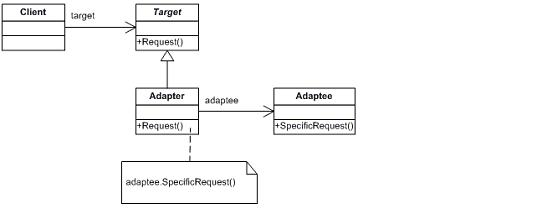
\includegraphics[scale=1]{img/IC104742}	
        \caption{classAdapter}
    \end{figure}

    \begin{itemize}
        \item \textbf{Target (Contact)}: Definisce l’interfaccia di riferimento alla quale l’oggetto Adaptee si deve adattare.
        \item \textbf{Adaptee (Employee)}: Rappresenta l’interfaccia che deve essere adattata.
        \item \textbf{Adapter (EmployeeAdapter)}: Adatta l’interfaccia di Adaptee all’interfaccia di Target.
        \item \textbf{Client (Program)}: Utilizza unicamente oggetti compatibili con l’interfaccia di Target.
    \end{itemize}
    
    \begin{figure}[h!] %img
        \centering
        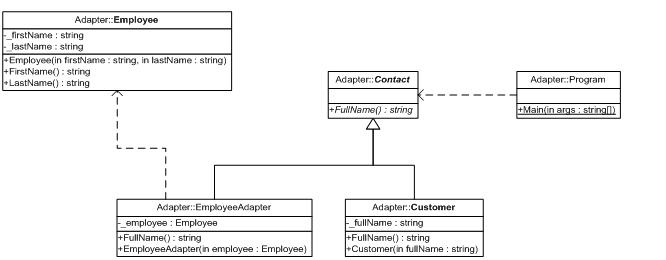
\includegraphics[scale=0.65]{img/IC53435}	
        \caption{esempio di classAdapter}
    \end{figure}
    \newpage
    \subsubsection{Esempio}
    Viene di seguito riportato un esempio applicativo di Design Pattern Adapter, utilizzato per interfacciare classi diverse altrimenti incompatibili.

        \begin{lstlisting}
            using System;
            using System.Collections.Generic;
            using System.Text;
            
            namespace DesignPatterns.Adapter
            {
                public class Employee
                {
                    private string _firstName;
                    private string _lastName;
            
                    public Employee(string firstName, string lastName)
                    {
                        _firstName = firstName; _lastName = lastName;
                    }
            
                    public string FirstName
                    {
                        get { return _firstName; }
                    }
            
                    public string LastName
                    {
                        get { return _lastName; }
                    }
                }
            
                public abstract class Contact
                {
                    public abstract string FullName { get; }
                }
            
                public class Customer : Contact
                {
                    private string _fullName;
            
                    public Customer(string fullName)
                    {
                        _fullName = fullName;
                    }
            
                    public override string FullName
                    {
                        get { return _fullName; }
                    }
                }
            
                public class EmployeeAdapter : Contact
                {
                    private Employee _employee;
            
                    public EmployeeAdapter(Employee employee)
                    {
                        _employee = employee;
                    }

                    public override string FullName
                    {
                        get { return _employee.FirstName + " " + _employee.LastName; }
                    }
                }
            
                public class Program
                {
                    public static void Main(string[] args)
                    {
                        Contact c = new Customer("Riccardo Golia");
                        Console.WriteLine(c.FullName);
                        c = new EmployeeAdapter(new Employee("Riccardo", "Golia"));
                        Console.WriteLine(c.FullName);
                        Console.ReadLine();
                    }
                }
            }
        \end{lstlisting}

    \newpage

    \subsection{Decorator}
    \subsubsection{Descrizione}
    Il decorator pattern è molto utile ed è utilizzato al posto della ereditarietà in situazioni in cui è necessario aggiungere/modificare a runtime il comportamento di un oggetto senza scomodare l’ereditarietà.    
    \begin{figure}[h!] %img
        \centering
        
\includegraphics[scale=0.75]{img/decorator}	
        \caption{classDecorator}
    \end{figure}

    \begin{itemize}
        \item \textbf{Component (Consumation)}: rappresenta l’interfaccia dell’oggetto che dovrà essere decorato dinamicamente;
        \item \textbf{ConcreteComponent (CheeseBurger)}: rappresenta l’oggetto a cui andranno aggiunte le nuove funzionalità,
        \item \textbf{Decorator (ExtraAdditionDecorator)}: rappresenta l’interfaccia tra il Component e i ConcreteDecorator,
        possiede un riferimento al Component e un’interfaccia a esso conforme,
        \item \textbf{ConcreteDecorator (ExtraMaioneseDecorator)}: rappresentano gli oggetti che aggiungono le
        nuove funzionalità ai ConcreteComponent.
    \end{itemize}
    
    \newpage
    \subsubsection{Esempio}
    Viene di seguito riportato un esempio applicativo di Design Pattern Decorator, utilizzato aggiugere la maionese alla classe cheeseburger.

        \begin{lstlisting}
            public abstract class Consumation {
                String productName = "";
                public String getProductName() {
                return productName;
                }
                public abstract double getPrice();
               }

               public class CheeseBurger extends Consumation {
                    public CheeseBurger() {
                        productName = "CheeseBurger";
                    }
                    @Override
                        public double getPrice() {
                        return 2.50;
                    }
               }

               public abstract class ExtraAdditionDecorator extends Consumation {
                protected Consumation consumation;
                @Override
                public abstract String getProductName();
               }

               public class ExtraMaioneseDecorator extends ExtraAdditionDecorator {
                public ExtraMaioneseDecorator(Consumation consumation){
                    this.consumation = consumation;
                }
                @Override
                public String getProductName() {
                    return consumation.getProductName()+ " con extra maionese";
                }
                @Override
                public double getPrice() {
                    return consumation.getPrice()+0.20;
                }
            }

            public class Main {
                    public static void main(String[] args) {
                    //CheeseBurger
                    Consumation cheeseburger = new CheeseBurger();
                    //voglio aggiungere la maionese al burger
                    Consumation hamburgerConMaionese = new ExtraMaioneseDecorator(cheeseburger);
                    System.out.println("Prodotto:" +
                    hamburgerConMaionese.getProductName() +
                    " di prezzo " + String.format("%.2f", hamburgerConMaionese.getPrice()));
               }
        \end{lstlisting}

        \newpage

        \subsection{Facade}
        \subsubsection{Descrizione}

        Il pattern Facade, di tipo strutturale basato sugli oggetti, permette di individuare un’interfaccia unificata per un insieme di interfacce nell’ambito di un sottosistema. Questo pattern in pratica consente di definire un’interfaccia a un livello più alto che semplifica l’accesso alle funzionalità erogate dal sottosistema e che fornisce un’entry-point unico al sottosistema stesso.
        \begin{figure}[h!] %img
            \centering
            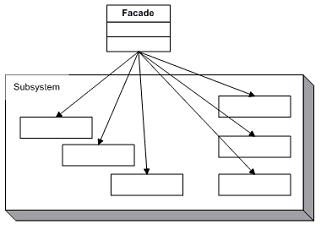
\includegraphics[scale=1]{img/IC94830}	
            \caption{classProxy}
        \end{figure}
    
        \begin{itemize}
            \item \textbf{Facade}: (SystemManager) Conosce la struttura del sottosistema e delega agli oggetti interni più appropriati la richieste provenienti dall’esterno;
            \item \textbf{Classi di Subsystem}: (SystemOne, SystemTwo e SystemThree) Forniscono le funzionalità interne adatte a rispondere alle richieste provenienti da Facade. Esse non hanno conoscenza dell’esistenza di Facade e non dipendono da esso;
        \end{itemize}
        
        \begin{figure}[h!] %img
            \centering
            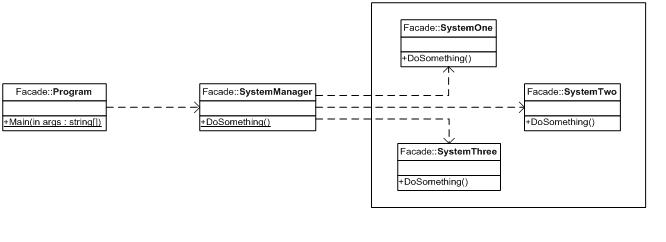
\includegraphics[scale=0.90]{img/IC101699}	
            \caption{esempio di classProxy}
        \end{figure}

        \newpage
        \subsubsection{Esempio}

Nell’esempio proposto l’interfaccia IService fornisce il contratto che deve essere rispettato sia dall’oggetto vero e proprio di tipo MyService, sia dal suo surrogato ServiceProxy. Tramite la classe factory ServiceFactory, il client attiva un’istanza della classe proxy che assegna a un riferimento di tipo IService. Il client peraltro non è consapevole di stare usando un surrogato, semplicemente richiama i membri definiti dal contratto, indipendentemente dal tipo concreto istanziato. La classe proxy permette di eseguire più codice rispetto all’oggetto originario: internamente al metodo HandleRequest() vengono infatti eseguite istruzioni prima e dopo la chiamata del metodo di destinazione. Nel caso dell’esempio il tipo di istruzioni aggiuntive incluse nella funzione sono davvero semplici, ma si può arrivare ad avere situazioni in cui il codice presente all’interno della classe proxy è molto più corposo e sostanzioso.
    
            \begin{lstlisting}
                using System;

                namespace DesignPatterns.Facade
                {
                    public static class SystemManager
                    {
                        public static void DoSomething()
                        {
                            new SystemOne().DoSomething();
                            new SystemTwo().DoSomething();
                            new SystemThree().DoSomething();
                        }
                    }
                
                    internal class SystemOne
                    {
                        public void DoSomething()
                        {
                            Console.WriteLine("One");
                        }
                    }
                
                    internal class SystemTwo
                    {
                        public void DoSomething()
                        {
                            Console.WriteLine("Two");
                        }
                    }
                
                    internal class SystemThree
                    {
                        public void DoSomething()
                        {
                            Console.WriteLine("Three");
                        }
                    }
                
                    public class Program
                    {
                        public static void Main(string[] args)
                        {
                            SystemManager.DoSomething();
                            Console.ReadLine();
                        }
                    }
                }
            \end{lstlisting}

            \subsection{Proxy}
            \subsubsection{Descrizione}
    
            Lo scopo del pattern Proxy (detto anche Surrogate) è quello di fornire un surrogato o un segnaposto di un altro oggetto per controllarne l’accesso. Questo pattern, di tipo strutturale basato sugli oggetti, è applicabile ogni volta che si voglia disporre di un riferimento a un oggetto più versatile di un semplice puntatore, tale da permettere, per esempio, di controllare l’accesso all’oggetto vero e proprio piuttosto che di fornire una rappresentazione locale di un oggetto remoto.

            \begin{figure}[h!] %img
                \centering
                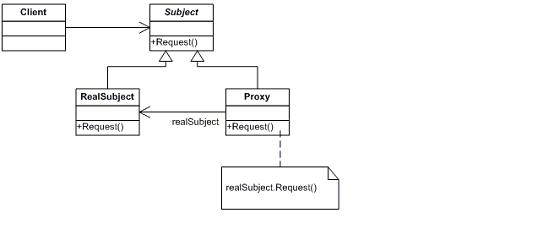
\includegraphics[scale=1]{img/IC119186}	
                \caption{classFacade}
            \end{figure}

            Il pattern in questione introduce un livello di indirezione nell’accesso a un oggetto. Questa indirezione ricopre significati diversi a seconda dei casi:
                    
            \begin{itemize}
                \item si parla di \textbf{proxy remoto} quando si vuole nascondere al client che un oggetto risiede in uno spazio di indirizzamento diverso (esempio classico: Web Service);
                \item si parla di \textbf{proxy virtuale} quando si vuole eseguire un’ottimizzazione nella creazione di un oggetto particolarmente “costoso” e pesante piuttosto che memorizzare informazioni aggiuntive relative all’oggetto rappresentato per posticipare l’accesso all’oggetto stesso;
                \item si parla di \textbf{proxy di protezione} quando si vuole gestire l’accesso a un oggetto tramite l’esecuzione di azioni preliminari di controllo.
                
            \end{itemize}
            
            \begin{figure}[h!] %img
                \centering
                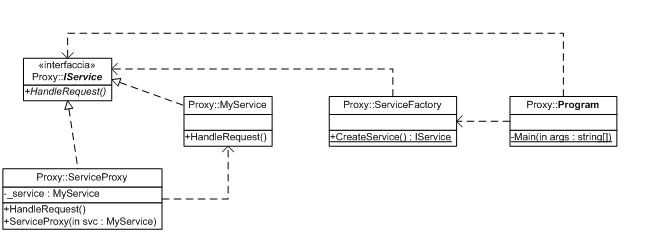
\includegraphics[scale=0.90]{img/IC119095}	
                \caption{esempio di classFacade}
            \end{figure}
    
            \newpage
            \subsubsection{Esempio}
            Nell’esempio proposto l’interfaccia IService fornisce il contratto che deve essere rispettato sia dall’oggetto vero e proprio di tipo MyService, sia dal suo surrogato ServiceProxy. Tramite la classe factory ServiceFactory, il client attiva un’istanza della classe proxy che assegna a un riferimento di tipo IService. Il client peraltro non è consapevole di stare usando un surrogato, semplicemente richiama i membri definiti dal contratto, indipendentemente dal tipo concreto istanziato. La classe proxy permette di eseguire più codice rispetto all’oggetto originario: internamente al metodo HandleRequest() vengono infatti eseguite istruzioni prima e dopo la chiamata del metodo di destinazione. Nel caso dell’esempio il tipo di istruzioni aggiuntive incluse nella funzione sono davvero semplici, ma si può arrivare ad avere situazioni in cui il codice presente all’interno della classe proxy è molto più corposo e sostanzioso.
                \begin{lstlisting}
                    using System;

                    namespace DesignPatterns.Proxy
                    {
                        public interface IService
                        {
                            void HandleRequest();
                        }
                    
                        public class MyService : IService
                        {
                            public void HandleRequest()
                            {
                                Console.WriteLine("Handling the request...");
                            }
                        }
                    
                        public class ServiceProxy : IService
                        {
                            private MyService _service;
                    
                            public ServiceProxy(MyService svc)
                            {
                                _service = svc;
                            }
                    
                            public void HandleRequest()
                            {
                                Console.WriteLine("Preprocessing by proxy...");
                                _service.HandleRequest();
                                Console.WriteLine("Postprocessing by proxy...");
                            }
                        }
                    
                        public static class ServiceFactory
                        {
                            public static IService CreateService()
                            {
                                return new ServiceProxy(new MyService());
                            }
                        }
                    
                        public class Program
                        {
                            static void Main(string[] args)
                            {
                                IService svc = ServiceFactory.CreateService();
                                svc.HandleRequest();
                                Console.ReadLine();
                            }
                        }
                    }
                \end{lstlisting}
            \newpage
            \section{Design pattern - CREAZIONALI}
                \subsection{Singleton}
                \subsubsection{Descrizione}
        


                Lo scopo del pattern Singleton è quello di assicurare che per una determinata classe esista un’unica istanza attiva, fornendo un entry-point globale all’istanza stessa. Questo pattern si può rivelare utile nel caso in cui si abbia la necessità di centralizzare informazioni e comportamenti in un’unica entità condivisa da tutti i suoi utilizzatori. La soluzione che più si adatta a risolvere la questione associata al pattern (unicità dell’istanza) consiste nell’associare alla classe stessa la responsabilità di creare le proprie istanze. In questo modo è la classe stessa che può assicurare che nessun’altra istanza possa essere creata, intercettando e gestendo in modo centralizzato le richieste di creazione di nuove istanze.    
                \begin{figure}[h!] %img
                    \centering
                    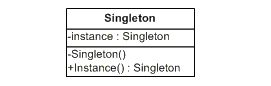
\includegraphics[scale=1]{img/IC18161}
                    \caption{classSingleton}
                \end{figure}
    
                Il pattern in questione introduce un livello di indirezione nell’accesso a un oggetto. Questa indirezione ricopre significati diversi a seconda dei casi:
                        
                \begin{itemize}
                    \item \textbf{Singleton}: (One, Two e Three) Definisce un membro per accedere all’unica istanza esistente, generalmente creata internamente alla classe stessa.
                    
                \end{itemize}
                
                \begin{figure}[h!] %img
                    \centering
                    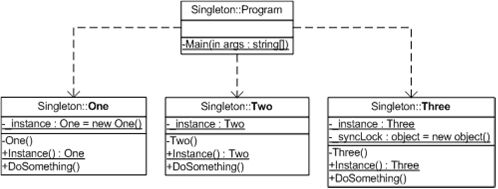
\includegraphics[scale=0.90]{img/IC20518}	
                    \caption{esempio di classSingleton}
                \end{figure}
        
                \newpage
                \subsubsection{Esempio}
                L’esempio proposto mostra tre casistiche diverse di applicazione del pattern. La classe One prevede l’inizializzazione statica dell’istanza. La proprietà Instance ritorna l’oggetto equivalente di tipo One statico e privato. La classe Two prevede l’inizializzazione dinamica su richiesta tramite il controllo del riferimento all’istanza. La proprietà Instance ritorna anche in questo caso l’oggetto equivalente di tipo Two statico e privato. La classe Three effettua un doppio controllo sul riferimento all’istanza, dentro e fuori ad un blocco a mutua esclusione e in base ad esso attiva l’istanza. Ancora una volta la proprietà Instance ritorna l’oggetto equivalente di tipo Three statico e privato. Se i primi due casi non sono thread-safe, il terzo lo è (nell’ambito di uno stesso appdomain). La presenza del blocco di mutua esclusione garantisce che la creazione dell’istanza sia effettivamente eseguita una volta sola, anche in un contesto multi-thread.
                    \begin{lstlisting}
                        using System;
                        using System.Threading;
                        
                        namespace DesignPatterns.Singleton
                        {
                            public sealed class One
                            {
                                private static One _instance = new One();
                                private One() {}
                        
                                public static One Instance
                                {
                                    get { return _instance; }
                                }
                        
                                public void DoSomething()
                                {
                                    Console.WriteLine("One");
                                }
                            } // One
                        
                            public sealed class Two
                            {
                                private static Two _instance;
                                private Two() {}
                        
                                public static Two Instance
                                {
                                    get
                                    {
                                        if (_instance == null)
                                            _instance = new Two();
                                        return _instance;
                                    }
                                }
                        
                                public void DoSomething()
                                {
                                    Console.WriteLine("Two");
                                }
                            } // Two
                        
                            public sealed class Three
                            {
                                private static Three _instance;
                                private static object _syncLock = new object();
                                private Three() {}
                        
                                public static Three Instance
                                {
                                    get
                                    {
                                        if (_instance == null)
                                            lock (_syncLock)
                                            {
                                                if (_instance == null)
                                                    _instance = new Three();
                                            } // lock
                                        return _instance;
                                    }
                                }
                        
                                public void DoSomething()
                                {
                                    Console.WriteLine("Three");
                                }
                            } // Three
                        
                            public class Program
                            {
                                static void Main(string[] args)
                                {
                                    One.Instance.DoSomething();
                                    Two.Instance.DoSomething();
                                    Three.Instance.DoSomething();
                                    Console.ReadLine();
                                }
                            }
                        }
                    \end{lstlisting}
                \newpage
                \subsection{Builder}
                \subsubsection{Descrizione}
                Il pattern Builder consente di dividere la costruzione di un oggetto complesso e composito dalla sua rappresentazione, in maniera tale che lo stesso processo di costruzione possa essere utilizzato per creare rappresentazioni diverse. L’applicazione di questo pattern si rivela assai indicata quando l’algoritmo di creazione dell’oggetto composito deve essere mantenuto distinto dalle parti costituenti e dal modo con cui esse sono unite insieme a formare un tutt’uno, consentendo un migliore controllo del processo di costruzione e isolando da tutto il resto il codice di assemblaggio.

                \begin{figure}[h!] %img
                    \centering
                    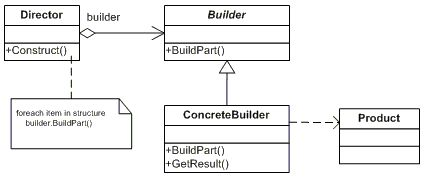
\includegraphics[scale=0.70]{img/IC106751}
                    \caption{classBuilder}
                \end{figure}
    
                I partecipanti di questo pattern sono:
                        
                \begin{itemize}
                    \item \textbf{Builder}: Rappresenta l’interfaccia di riferimento (generalmente astratta) per la creazione delle parti costituenti l’oggetto da costruire.
                    \item \textbf{ConcreteBuilder}: (Wheel, Engine e Chassis) Genera e costruisce ogni singola parte concreta dell’oggetto composito tramite l’implementazione di Builder. Definisce un metodo di costruzione BuildPart e uno di accesso al risultato della costruzione GetResult.
                    \item \textbf{Director}: (CarBuilder) Assembla l’oggetto utilizzando l’interfaccia Builder. Infatti il client (Program) istanzia questo oggetto configurandolo in maniera tale da farlo operare con l’oggetto Builder desiderato.
                    \item \textbf{Product}: (Car) Rappresenta l’oggetto composito che è il risultato dell’operazione di costruzione e assemblaggio.
                    
                \end{itemize}
                
                \begin{figure}[h!] %img
                    \centering
                    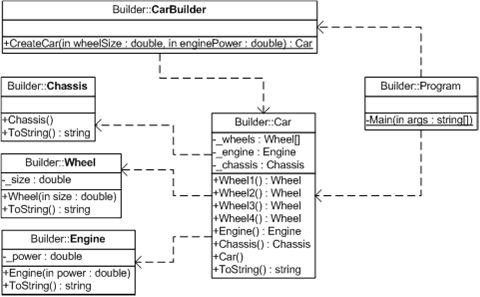
\includegraphics[scale=0.5]{img/IC103594}	
                    \caption{esempio di classBuilder}
                \end{figure}
        
                \newpage
                \subsubsection{Esempio}
                Quello proposto è un esempio molto semplificato di applicazione del pattern in questione. Si tratta della costruzione di un oggetto di tipo Car che comprende quattro proprietà, ovvero un array composto da 4 elementi di tipo Wheel (ruota), un Engine (motore) e un Chassis (telaio). Ciascuna di queste parti implementa in modo particolare il metodo ToString di System.Object (lo possiamo considerare come l’equivalente del metodo GetResult nella rappresentazione generale) e definisce un costruttore, accettando eventuali parametri utili alla creazione delle singole istanze (lo possiamo pensare come l’equivalente del metodo BuildPart nella rappresentazione generale). L’oggetto che è incaricato di costruire l’assemblato è la classe CarBuilder che, tramite il metodo statico CreateCar, accetta i parametri di costruzione validi per le diverse parti e chiama i costruttori per la generazione delle istanze. Il metodo ToString della classe Car richiama internamente i metodi ToString delle parti costituenti per ottenere una rappresentazione completa dell’oggetto. 
                    \begin{lstlisting}
                        using System;

                        namespace DesignPatterns.Builder
                        {
                            public class Car
                            {
                                private Wheel[] _wheels;
                                private Engine _engine;
                                private Chassis _chassis;
                        
                                public Wheel Wheel1
                                {
                                    set { _wheels[0] = value; }
                                    get { return _wheels[0]; }
                                }
                        
                                public Wheel Wheel2
                                {
                                    set { _wheels[1] = value; }
                                    get { return _wheels[1]; }
                                }
                        
                                public Wheel Wheel3
                                {
                                    set { _wheels[2] = value; }
                                    get { return _wheels[2]; }
                                }
                        
                                public Wheel Wheel4
                                {
                                    set { _wheels[3] = value; }
                                    get { return _wheels[3]; }
                                }
                        
                                public Engine Engine
                                {
                                    set { _engine = value; }
                                    get { return _engine; }
                                }
                        
                                public Chassis Chassis
                                {
                                    set { _chassis = value; }
                                    get { return _chassis; }
                                }
                        
                                public Car()
                                {
                                  _wheels = new Wheel[4];
                                }
                        
                                public override string ToString()
                                {
                                    return _wheels[0].ToString() + " / " +
                                           _wheels[1].ToString() + " / " +
                                           _wheels[2].ToString() + " / " +
                                           _wheels[3].ToString() + " / " +
                                           _engine.ToString() + " / " + _chassis.ToString();
                                }
                            }
                        
                            public class Wheel
                            {
                                private double _size;
                        
                                public Wheel(double size) { _size = size; }
                        
                                public override string ToString()
                                {
                                    return "Wheel " + _size.ToString();
                                }
                            }
                        
                            public class Engine
                            {
                                private double _power;
                        
                                public Engine(double power) { _power = power; }
                        
                                public override string ToString()
                                {
                                    return "Engine " + _power.ToString();
                                }
                            }
                        
                            public class Chassis
                            {
                                public Chassis() {}
                        
                                public override string ToString()
                                {
                                    return "Chassis";
                                }
                            }
                        
                            public class CarBuilder
                            {
                                public static Car CreateCar(double wheelSize, double enginePower)
                                {
                                    Car c = new Car();
                                    c.Wheel1 = new Wheel(wheelSize);
                                    c.Wheel2 = new Wheel(wheelSize);
                                    c.Wheel3 = new Wheel(wheelSize);
                                    c.Wheel4 = new Wheel(wheelSize);
                                    c.Engine = new Engine(enginePower);
                                    c.Chassis = new Chassis();
                                    return c;
                                }
                            }
                        
                            public class Program
                            {
                                static void Main(string[] args)
                                {
                                    Console.WriteLine(CarBuilder.CreateCar(180, 110).ToString());
                                    Console.ReadLine();
                                }
                            }
                        }
                    \end{lstlisting}
                    \newpage
                    \subsection{Abstract Factory}
                    \subsubsection{Descrizione}
                    L’Abstract Factory (detto anche Kit) è un pattern creazionale che ha lo scopo di fornire un’interfaccia per la creazione di famiglie di oggetti tra loro correlati o dipendenti limitando l’accoppiamento derivante dall’uso diretto delle classi concrete. L’applicazione di questo pattern si rivela assai utile quando si vuole rendere un sistema indipendente dalle modalità di creazione, composizione e rappresentazione degli oggetti costituenti, rendendo note unicamente le interfacce e non le implementazioni concrete. Questo consente di rendere tra loro interscambiabili le diverse implementazioni che soddisfano una determinata interfaccia, senza che il contesto d’uso dell’istanza debba essere modificato al variare dell’implementazione scelta.
    
                    \begin{figure}[h!] %img
                        \centering
                        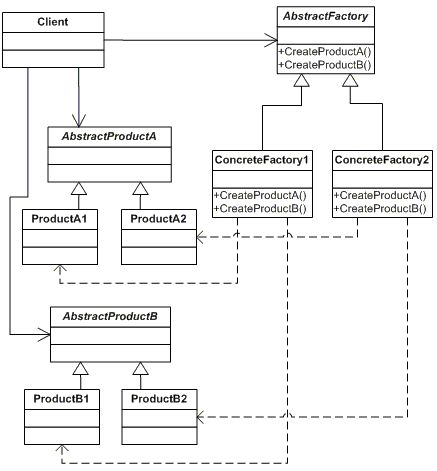
\includegraphics[scale=0.50]{img/IC92016}
                        \caption{classAbstractFactory}
                    \end{figure}
        
                    I partecipanti di questo pattern sono:
                            
                    \begin{itemize}
                        \item \textbf{AbstractFactory}: (IShapeFactory) Definisce l’interfaccia di riferimento per gli oggetti che creano le istanze.
                        \item \textbf{ConcreteFactory}: (MyShapeFactory) Implementa in modo concreto l’interfaccia definita da AbstractFactory e crea effettivamente una tipologia specifica di oggetti appartenenti ad una famiglia.
                        \item \textbf{AbstractProduct}: (Circle e Rectangle) Definisce l’interfaccia di riferimento per una famiglia di oggetti da creare tramite il factory corrispondente.
                        \item \textbf{ConcreteProduct}: (MyCircle e MyRectangle) Implementa in modo concreto l’oggetto appartenente alla famiglia per cui vale l’interfaccia AbstractProduct e che viene creato dall’oggetto factory corrispondente.
                        \item \textbf{Client}: (Program) Utilizza unicamente le classi astratte del factory e dell’oggetto da creare, senza conoscerne gli aspetti implementativi. L’annullamento dell’accoppiamento tra il client e gli oggetti concreti è ottenuto tramite l’inversione delle dipendenze, uno dei principi base dell’Object Oriented Design (OOD).
                    \end{itemize}
                    
                    \begin{figure}[h!] %img
                        \centering
                        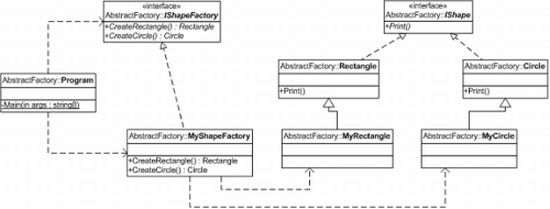
\includegraphics[scale=0.75]{img/IC130807}	
                        \caption{esempio di classAbstractFactory}
                    \end{figure}
            
                    \newpage
                    \subsubsection{Esempio}
                    L’esempio proposto per questo pattern include innanzitutto un’interfaccia IShape (forma) che dichiara un metodo Print che deve essere presente in tutte le istanze che la implementano. In particolare queste istanze sono rappresentate dagli oggetti di tipo MyCircle e MyRectangle, che implementano l’interfaccia IShape in modo indiretto tramite le classi base Circle e Rectangle rispettivamente. L’oggetto MyShapeFactory implementa l’interfaccia IShapeFactory e nei metodi CreateCircle e CreateRectangle crea tramite il costruttore di default le istanze di tipo MyCircle e MyRectangle. Nel client (Program) non viene fatto alcun riferimento alle classi MyCircle e MyRectangle. Dal momento che il client non conosce in modo diretto i tipi effettivamente creati dal factory, qualsiasi dipendenza di Program dai tipi concreti effettivamente utilizzati al suo interno viene eliminata.
                        \begin{lstlisting}
                            using System;

                            namespace DesignPatterns.AbstractFactory
                            {
                                public interface IShape 
                                {
                                    void Print();
                                }
                            
                                public class Rectangle : IShape
                                {
                                    public virtual void Print()
                                    {
                                        Console.WriteLine("Rectangle");
                                    }
                                }
                            
                                public class Circle : IShape
                                {
                                    public virtual void Print()
                                    {
                                        Console.WriteLine("Circle");
                                    }
                                }
                            
                                public interface IShapeFactory
                                {
                                    Rectangle CreateRectangle();
                                    Circle CreateCircle();
                                }
                            
                                public class MyRectangle : Rectangle
                                {
                                    public override void Print()
                                    {
                                        Console.WriteLine("MyRectangle");
                                    }
                                }
                            
                                public class MyCircle : Circle
                                {
                                    public override void Print()
                                    {
                                        Console.WriteLine("MyCircle");
                                    }
                                }
                            
                                public class MyShapeFactory : IShapeFactory
                                {
                                    public Rectangle CreateRectangle()
                                    {
                                        return new MyRectangle();
                                    }
                            
                                    public Circle CreateCircle()
                                    {
                                        return new MyCircle();
                                    }
                                }
                            
                                public class Program
                                {
                                    static void Main(string[] args)
                                    {
                                        IShapeFactory fac = new MyShapeFactory();
                                        Circle c = fac.CreateCircle();
                                        Rectangle r = fac.CreateRectangle();
                                        c.Print();
                                        r.Print();
                                        Console.ReadLine();
                                    }
                                }
                            }
                            
                        \end{lstlisting}
                        \newpage
                        \section{Design pattern - COMPORTAMENTALI}
                        \subsection{Command}
                        \subsubsection{Descrizione}
                        Il pattern Command (noto anche come Action o Transaction) permette di inoltrare richieste ad oggetti senza conoscere assolutamente nulla dell’operazione da eseguire o del destinatario della richiesta. Questo è possibile per il fatto che il pattern in questione tratta la richiesta come un oggetto differente rispetto sia al richiedente che all’oggetto destinatario. Questo oggetto specifica l’azione da svolgere sul destinatario, sfruttandone i comportamenti in modo da tale da poter portare a termine la richiesta.
                        \begin{itemize}
                            \item per parametrizzare gli oggetti rispetto ad una azione da compiere;                            
                            \item per specificare, accodare ed eseguire svariate richieste in tempi diversi, anche trasferendo un comando da un contesto di esecuzione ad un altro;
                            \item per consentire l’annullamento delle operazioni eseguite (undo, rollback), mantenendo preventivamente lo stato per annullare gli effetti dei comandi stessi.
                        \end{itemize}
                        Il vantaggio più significativo nell’applicazione di questo pattern è il fatto di ottenere un perfetto disaccoppiamento tra l’oggetto che invoca il comando e il destinatario, ovvero quello che conosce il modo per portare a termine l’operazione. Questo aspetto consente di poter aggiungere comandi ulteriori associati a destinatari diversi in modo abbastanza immediato senza che sia necessario modificare le classi già esistenti. Inoltre il fatto che i comandi siano oggetti distinti permette di poterli eventualmente aggregare insieme (applicando il pattern Composite) allo scopo di formare un comando complesso, costituito da una serie arbitraria di azioni.

                        \begin{figure}[h!] %img
                            \centering
                            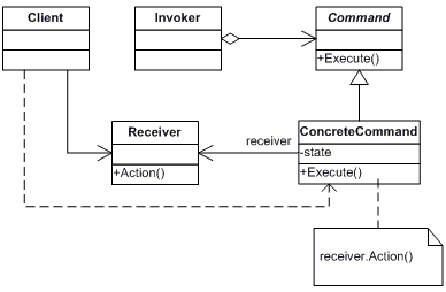
\includegraphics[scale=0.50]{img/IC138773}
                            \caption{classAbstractFactory}
                        \end{figure}
                        I partecipanti di questo pattern sono (tra parentesi sono indicati gli oggetti equivalenti nell’esempio proposto successivamente):
                            
                        \begin{itemize}
                            \item \textbf{Command}: (ICommand) Definisce l’interfaccia di riferimento per ogni comando.
                            \item \textbf{ConcreteCommand}: (Open, Read, Write e Close) Definisce un legame tra il Receiver e un’azione. Implementa in modo particolare il metodo Execute() invocando i metodi del Receiver.
                            \item \textbf{Invoker}: (Reader e Writer) Aggrega i diversi comandi e delega a loro l’esecuzione delle azioni previste.
                            \item \textbf{Receiver}: (System.Console) Conosce il modo di eseguire le operazioni associate ad una particolare richiesta.
                            \item \textbf{Client}: (Program) Tramite l’Invoker attiva ed esegue un ConcreteCommand che va a interessare il Receiver corrispondente.
                        \end{itemize}
                        
                        \begin{figure}[h!] %img
                            \centering
                            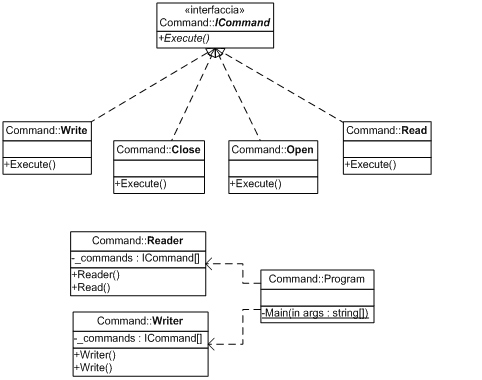
\includegraphics[scale=0.75]{img/IC65512}	
                            \caption{esempio di classAbstractFactory}
                        \end{figure}
                
                        \newpage
                        \subsubsection{Esempio}
                        L’esempio proposto si riferisce all’esecuzione di due sequenze di comandi da parte delle classi Reader e Writer. L’esecuzione di ciascuna azione consiste nella scrittura sulla console di una stringa contenente il nome di ciascun comando appartenente alla sequenza. L’oggetto di destinazione pertanto è System.Console: Reader e Writer portano a compimento le operazioni desiderate sfruttando il suo metodo WriteLine(string). I singoli comandi sono classi diverse che implementano in modo particolare il metodo Execute(), definito nell’interfaccia ICommand. Si noti come il client (classe Program) sia completamente all’oscuro sia di come ciascun comando viene eseguito, sia di quale sequenza effettiva di azioni viene intrapresa di volta in volta.
                            \begin{lstlisting}
                                using System;

                                namespace DesignPatterns.Command
                                {
                                    public interface ICommand
                                    {
                                        void Execute();
                                    }
                                
                                    public class Open : ICommand
                                    {
                                        public virtual void Execute()
                                        {
                                            Console.WriteLine("Open");
                                        }
                                    }
                                
                                    public class Read : ICommand
                                    {
                                        public virtual void Execute()
                                        {
                                            Console.WriteLine("Read");
                                        }
                                    }
                                    
                                    public class Write : ICommand
                                    {
                                        public virtual void Execute()
                                        {
                                            Console.WriteLine("Write");
                                        }
                                    }
                                
                                    public class Close : ICommand
                                    {
                                        public virtual void Execute()
                                        {
                                            Console.WriteLine("Close");
                                        }
                                    }
                                
                                    public class Reader
                                    {
                                        private ICommand[] _commands;
                                
                                        public Reader()
                                        {
                                            _commands = new ICommand[] { new Open(), new Read(), new Close() };
                                        }
                                
                                        public void Read()
                                        {
                                            foreach (ICommand cmd in _commands)
                                                cmd.Execute();
                                        }
                                    }
                                
                                    public class Writer
                                    {
                                        private ICommand[] _commands;
                                
                                        public Writer()
                                        {
                                            _commands = new ICommand[] { new Open(), new Write(), new Close() };
                                        }
                                
                                        public void Write()
                                        {
                                            foreach (ICommand cmd in _commands)
                                                cmd.Execute();
                                        }
                                    }
                                
                                    public class Program
                                    {
                                        static void Main(string[] args)
                                        {
                                            Reader reader = new Reader();
                                            reader.Read();
                                            Writer writer = new Writer();
                                            writer.Write();
                                            Console.ReadLine();
                                        }
                                    }
                                }
                            \end{lstlisting}
                            \newpage
                            \subsection{Observer}
                            \subsubsection{Descrizione}
                            Il pattern Observer (noto anche col nome Publish-Subscribe) permette di definire una dipendenza uno a molti fra oggetti, in modo tale che se un oggetto cambia il suo stato interno, ciascuno degli oggetti dipendenti da esso viene notificato e aggiornato automaticamente. L’Observer nasce dall’esigenza di mantenere un alto livello di consistenza fra classi correlate, senza peraltro produrre situazioni di forte dipendenza e accoppiamento elevato.

                            Il pattern Observer si presta ad essere utilizzato in diversi casi. Ad esempio, quando un’astrazione presenta due diversi aspetti tra loro dipendenti, è possibile definire due classi in cui incapsulare questi aspetti in modo tale da poterli utilizzare in maniera indipendente. In questo scenario occorre comunque prevedere un meccanismo di comunicazione che permetta di mantenere la consistenza tra le istanze delle due classi e il pattern Observer fornisce una soluzione elegante al problema senza generare accoppiamento. Un’altra situazione tipica di utilizzo si ha quando la modifica dello stato di un oggetto (per esempio, un controllo dell’interfaccia utente) implica un cambiamento dello stato di altri oggetti correlati, a prescindere dal loro numero (per esempio, altri controlli). In questo caso la modifica dello stato dell’oggetto (detto anche Publisher) si deve propagare agli oggetti correlati (detti anche Subscriber) in modo tale che essi possano aggiornare il loro stato interno di conseguenza.
    
                            \begin{figure}[h!] %img
                                \centering
                                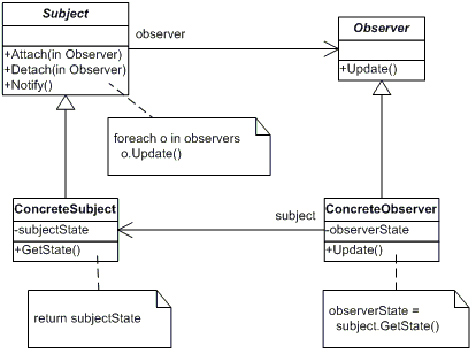
\includegraphics[scale=0.50]{img/IC68568}
                                \caption{classObserver}
                            \end{figure}
                            I partecipanti di questo pattern sono:
                                
                            \begin{itemize}
                                \item \textbf{Subject}: (delegate Subject.Notify) Conosce i suoi Observer. Fornisce l’interfaccia per associare e rimuovere oggetti Observer.
                                \item \textbf{Observer}: Fornisce l’interfaccia di notifica per gli oggetti a cui devono essere segnalati i cambiamenti di stato di Subject.
                                \item \textbf{ConcreteSubject}: (Subject) Contiene lo stato monitorato dagli Observer a cui viene inviata la notifica.
                                \item \textbf{ConcreteObserver}: (Observer) Mantiene un riferimento ad un oggetto ConcreteSubject. Contiene le informazioni da mantenere sincronizzate con lo stato del Subject. Implementa il metodo di gestione della notifica da eseguire allo scopo di mantenere sincronizzati gli stati degli oggetti.
                            \end{itemize}
                            
                            \begin{figure}[h!] %img
                                \centering
                                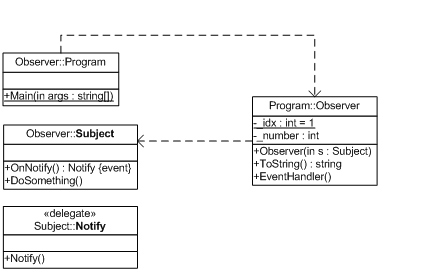
\includegraphics[scale=0.75]{img/IC51233}	
                                \caption{esempio di classObserver}
                            \end{figure}
                    
                            \newpage
                            \subsubsection{Esempio}
                            Il meccanismo per inviare notifiche nell’ambito del .NET Framework è fornito in modo nativo dai tipi delegate e dagli eventi. Una classe che funge da Publisher (classe Subject) espone in generale sulla sua interfaccia una serie di eventi corrispondenti ad un tipo particolare di delegate. Le classi Subscriber (classe Observer) sottoscrivono l’evento e ad esso associano un metodo interno (comunemente detto event handler) che deve rispettare la firma definita dal tipo delegate associato all’evento. L’event handler viene chiamato nel momento in cui il Publisher inoltra ai suoi Subscriber la notifica, rendendo possibile in questo modo l’esecuzione di codice in ciascun Subscriber al variare dello stato interno del Publisher.
                                \begin{lstlisting}
                                    using System;

                                    namespace DesignPatterns.Observer
                                    {
                                        public class Subject
                                        {
                                            public delegate void Notify();
                                    
                                            public event Notify OnNotify;
                                    
                                            public void DoSomething()
                                            {
                                                if (OnNotify != null)
                                                {
                                                    Console.WriteLine("Subject fires event");
                                                    OnNotify();
                                                }
                                            }
                                        }
                                    
                                        public class Program
                                        {
                                            public class Observer
                                            {
                                                private static int _idx = 1;
                                                private int _number;
                                    
                                                public Observer(Subject s)
                                                {
                                                    s.OnNotify += new Subject.Notify(EventHandler);
                                                    _number = _idx++;
                                                }
                                    
                                                public override string ToString()
                                                {
                                                    return _number.ToString();
                                                }
                                    
                                                public void EventHandler()
                                                {
                                                    Console.WriteLine("Observer {0} was called by subject", this);
                                                }
                                            }
                                    
                                            public static void Main(string[] args)
                                            {
                                                Subject s = new Subject();
                                                Observer o1 = new Observer(s);
                                                Observer o2 = new Observer(s);
                                                s.DoSomething();
                                                Console.ReadLine();
                                            }
                                        }
                                    }                                \end{lstlisting}
    
                        \end{document}